\typeout{IJCAI-11 Instructions for Authors}
\documentclass{article}
\usepackage{SortingNetworks}
\usepackage{times}
\usepackage{latexsym} 
\usepackage{pgfplots} % LaTeX
\usepackage{capt-of}
\usepackage[dutch]{babel}
\usepackage{amsthm}
\usetikzlibrary{arrows,automata}
\newtheorem{lemma}{Lemma}
\newtheorem{definitie}{Definitie}

\title{Sorteernetwerken van Optimale Grootte}%\thanks{Dankwoord}}
\author{Mathias Dekempeneer, Vincent Derkinderen \\
Bachelor Informatica\\
Katholieke Universiteit Leuven \\
{voornaam.achternaam}@student.kuleuven.be}

\begin{document}

\maketitle

\begin{abstract}
Korte samenvatting van wat we doen en wat de conclusie is.\\
Verder werken op paper van Codish et al. Sorteer optimal size sorting network.\\
Tijdsverbetering van x?
Bla\\
Bla\\
Bla\\
Bla\\
Bla\\
Bla\\
Bla\\
Bla\\
Bla\\
Bla\\
Bla\\
\end{abstract}

\section{Introductie}

Situering + bijdrage.\\
Sorting Network (high level), Optimal Size (high level), contributies andere papers rond deze twee, enkele getallen rond grootte orde van het probleem, wat er al geprobeerd is (SAT, generate \& prune,...), hoe wij het probleem zullen aanpakken (hoe wij prunen (high level)), gebruikte hardware...\\
Bla\\
Bla\\
Bla\\
Bla\\
Bla\\
Bla\\
Bla\\
Bla\\
Bla\\
Bla\\
Bla\\
Bla\\
Bla\\
Bla\\
Bla\\
Bla\\

\section{Probleemstelling}
Een \textit{comparator netwerk} $C^n_k$ bestaat uit $n$ kanalen en $k$ \textit{comparatoren}.
Een comparator $\left(i, j\right)$ verbindt twee verschillende kanalen $i$ en $j$ waarbij $0 < i < j \leq n$.
We nemen $x_l^m$ als waarde op kanaal $m$ net voor comparator $l$.
De $l^{de}$ comparator  vergelijkt de huidige waarden van beide kanalen en plaatst de kleinste waarde op kanaal $i$ en de grootste waarde op kanaal $j$ zodat $x_{l+1}^i = \min(x_l^i,x_l^j)$ en $x_{l+1}^j = \max(x_l^i,x_l^j)$.
De uitvoer van een comparator netwerk verwijst naar de partieel geordende vector $\vec{x} = \{x^1_{k+1} \dots x^n_{k+1} \} $. %TODO voeg toe: "elementen uit een totaal geordende set", invoer

Een \textit{sorteernetwerk} is een comparator netwerk met als eigenschap dat de uitvoer gesorteerd is ongeacht de invoer.
Een sorteernetwerk $C^n_k$ van optimale grootte houdt in dat er geen ander sorteernetwerk $C^n_l$ bestaat waarbij $l < k$. %TODO grootte = aantal comparatoren
Figuur \ref{Werking} is een voorbeeld van zo een netwerk waarop ook de werking gedemonstreerd wordt.
\begin{figure}[h!]
\centering
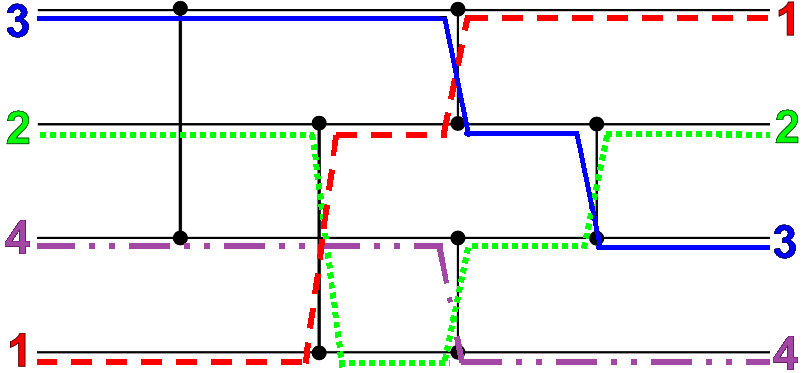
\includegraphics[scale=0.275]{NetworkTransparent.png} 
\caption{Sorteernetwerk 4 kanalen, 5 comparatoren}
\label{Werking}
\end{figure}
%TODO Hard enter?
Om te onderzoeken of een comparator netwerk een sorteernetwerk is, kunnen we gebruik maken van het \textit{nul - \'e\'en principe}. 
Dit principe, zoals beschreven volgens Knuth \cite{Knuth3}, stelt dat wanneer een comparator netwerk met $n$ kanalen alle $2^n$ mogelijke sequenties van $n$ $0$- en $1$-en sorteert, het een sorteernetwerk is.
De optimale grootte van een sorteernetwerk met $n$ kanalen is reeds bewezen tot en met $n \leq 10$ (Tabel \ref{tabel1} \cite{sortingNetworksSize2014}).
\begin{table}[h!]
\centering
\begin{tabular}{r|c|c|c|c|c|c|c}
n & 6 & 7 & 8 & 9 & 10 & 11 & 12\\ 
\hline 
bovengrens & 12 & 16 & 19 & 25 & 29 & 35 & 39\\ 
\hline 
ondergrens & 12 & 16 & 19 & 25& 29 & 33 & 37\\
\end{tabular} 
\caption{Minimaal aantal comparatoren bij $6 \leq n \leq 12$ kanalen.}
\label{tabel1}
\end{table}
%TODO Hard enter?
Voor $n > 10$ zijn er bovengrenzen gekend door zowel concrete voorbeelden als de systematische constructie van Batcher \cite{sortingNetworksApplications}. 
De ondergrenzen werden gevonden via bewijzen en lemma \ref{lemma1} \cite{Voorhis1972}.
\begin{lemma}
$S(n+1) \geq S(n) + \lceil \log_2(n) \rceil, \forall n \geq 1$
\label{lemma1}
\end{lemma}

\section{Voorgestelde oplossing}
Om te bewijzen dat een sorteernetwerk $C^n_k$ een sorteernetwerk is van optimale grootte, moeten we bewijzen dat er geen sorteernetwerk $C^n_{k-1}$ bestaat.
$n$ kanalen zorgen voor $\frac{n \left(n-1\right)}{2}$ verschillende comparatoren.
Wanneer een netwerk $k$ comparatoren bevat, kunnen er $\left(\frac{n \left(n-1\right)}{2}\right) ^k$ verschillende netwerken gevormd worden.
Voor $9$ kanalen en $24$ comparatoren betekent dit $2.245 \times 10^{37}$ verschillende netwerken, dit maakt het overlopen van alle netwerken niet aantrekkelijk.
%TODO Aaneenpraten
Door gebruik te maken van symmetrie\"en willen we snoeien in het aanmaken van deze netwerken.

We gebruiken de \textit{genereer- en snoei-methode} zoals beschreven door Codish \textit{et al.} (sectie 3, \cite{sortingNetworksSize2014}).
Deze methode heeft een cyclisch verloop waarbij men bij elke cyclus de set $R^n_k$ uitbreidt naar $N^n_{k+1}$ om vervolgens te snoeien en de set $R^n_{k+1}$ te bekomen (Figuur \ref{GenereerSnoei}).
\begin{figure}[!h]
\centering
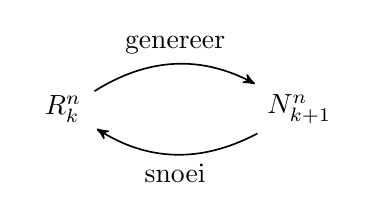
\begin{tikzpicture}[->,>=stealth',shorten >=1pt,auto,node distance=3cm,semithick]
  \tikzstyle{every state}=[fill=white,draw=none,text=black]

  \node[state] (A)                    {$R^n_k$};
  \node[state] (B) [right of=A] {$N^n_{k+1}$};

  \path (A) edge [bend left] node {genereer} (B)
  		  (B) edge [bend left] node {snoei} (A);
\end{tikzpicture}
\caption{Genereer en snoei principe}
\label{GenereerSnoei}
\end{figure}
Specifiek zullen we vertrekken van een netwerk zonder comparatoren om te eindigen bij $R^n_k$ bestaande uit \'e\'en sorteernetwerk van optimale grootte.
Bij de genereer-stap zullen we aan elk netwerk van $R^n_k$ alle mogelijke comparatoren toevoegen zodat $|N^n_{k+1}| = |R^n_{k}| \times \frac{n\left(n-1\right)}{2}$.
%TODO aanelkaarpraten zin misschien aanpassen)
Bij de snoei-stap zullen we dan netwerken verwijderen volgens het subsumes principe beschreven in definitie \ref{definitie1}.
Concreet kunnen we de definitie van subsumes en lemma \ref{lemma2} beschreven door Codish \textit{et al.} \cite{sortingNetworksSize2014} gebruiken om in te zien dat we netwerken die gesubsumed worden door andere netwerken kunnen verwijderen.
\begin{definitie}[Subsumes] %TODO VRAGEN SUBSUMES => TOM NEDERLANDS/ENGELS
We zeggen ``Comparator netwerk $C^n_{k,a}$ subsumes comparator netwerk $C^n_{k,b}$'' wanneer een permuntatie $\pi$ bestaat zodat $\pi\left(outputs\left(C_{a}\right)\right) \subseteq outputs\left(C_{b}\right)$. Dit wordt genoteerd als $ C_{a} \preceq C_{b}$ om aan te duiden dat er een permutatie $\pi$ bestaat zodat $C_{a}\leq_\pi C_{b}$. %TODO Vincent weent om dit te kunnen herzien
\label{definitie1}
\end{definitie}
\begin{lemma}
%TODO 
\label{lemma2}
\end{lemma}
Op deze manier zien we dat in de snoei-stap voor elke equivalentie klasse van minimale netwerken slechts \'e\'en representatief netwerk wordt bijgehouden.

~\\\\
Ontwerp, wat (algoritme)\\
Generate \& prune (en hoe we dit doen) + de getallen hier rond (zoals aantal comparatoren). Het prune idee uitleggen. Benadruk de slechte grootte orde en de nood aan snellere beslissingen om de uitkomst van de prune check op voorhand te weten.

\subsection{Representatie van sorteernetwerken}
Bijgehouden informatie van netwerken

\subsection{Genereren}
Uitleg hoe we de generate doen.\\
Redundant (of de comparator die je toevoegt, wel iets verandert? Uitleggen wat wij specifiek doen), unique\_if uitleggen

\subsection{Snoeien}
Uitleg hoe we de prune doen.\\
Checken  van alle netwerken met alle netwerken voor de prune stap.
\begin{itemize}
\item Aantal 1en bij $C_a > C_b \Rightarrow C_a$ subsumes niet $C_b$ 
\item $|W(C_a, x, k)| > |W(C_b, x, k)| \Rightarrow C_a$ subsumes niet $C_b$
\item Uitleggen reductie van permutaties
\end{itemize}

\subsection{Parallellisatie}
Parallellisatie uitleggen\\
Uitleg hoe generate and prune verandert door elke thread zijn stuk te laten generate en prunen en vervolgens in een groter geheel te prunen en hoe dit groter geheel prunen werkt zonder locks.
%TODO ZIe pagina 4 in paper => definitie 2: Observe that ......

\section{Evaluatie}
Empirische evaluaties + grafiekjes\\
Tabel geven van hoeveel beslissingen er op welke plaats genomen worden.\\ \\
Vergelijken runtime voor 9 kanalen met Codish.\\
Schatting runtime voor 10 kanalen.\\\\

\begin{figure}[!h]
\centering
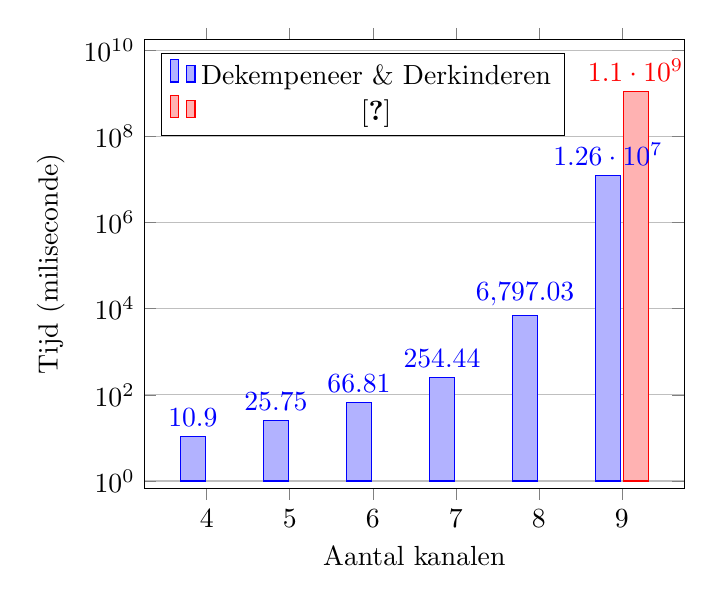
\begin{tikzpicture} 
	\begin{axis}[
		ylabel = Tijd (miliseconde),
		xlabel = Aantal kanalen,
		enlargelimits=0.15,
		ybar=1pt,
		ymode = log,
		log basis y = 10,
		bar width=9pt,
		nodes near coords,
		point meta=10^y,
		ymajorgrids = true, 
		legend pos = north west
]
%\addplot
%    coordinates {(4, 16.93) (5, 25.05) (6, 82.44) (7, 141.48) (8, 6680.31) (9, 15135358.01)};

\addplot
	coordinates {(4, 10.9026077) (5, 25.748741) (6, 66.820104) (7, 254.444729) (8, 6797.797437) (9, 12615521.409224)};	
	
\addplot
	coordinates {(9, 1101480000)};
	
\legend{Dekempeneer \& Derkinderen, \cite{sortingNetworksSize2014}};
\end{axis}
\end{tikzpicture}
\caption{Resultaten}
\end{figure}

\begin{figure}[!h]
\centering
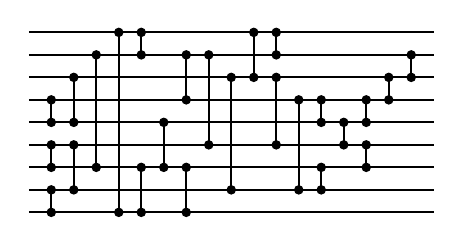
\begin{tikzpicture}
%\fill [gray!15] (1.5,1.5) -- (2.5,1.5) -- (2.5,2.5) -- (1.5,2.5) -- cycle;
%\foreach \a in {1,..,9}
\def\x{3.5}
\foreach \a in {1/\x, 2/\x, 3/\x, 4/\x, 5/\x, 6/\x, 7/\x, 8/\x, 9/\x}
  \draw[thick] (0,\a) -- ++(18/\x,0);
\foreach \b in {{1/\x,1/\x},{1/\x,2/\x},{1/\x,3/\x},{1/\x,4/\x},{1/\x,5/\x},{1/\x,6/\x},{2/\x,2/\x},{2/\x,4/\x},{2/\x,5/\x},{2/\x,7/\x},{3/\x,3/\x},{3/\x,8/\x},{4/\x,1/\x},{4/\x,9/\x},{5/\x,8/\x},{5/\x,9/\x},{5/\x,1/\x},{5/\x,3/\x},{6/\x,3/\x},{6/\x,5/\x},{7/\x,1/\x},{7/\x,3/\x},{7/\x,6/\x},{7/\x,8/\x},{8/\x,4/\x},{8/\x,8/\x},{9/\x,2/\x},{9/\x,7/\x},{10/\x,7/\x},{10/\x,9/\x},{11/\x,8/\x},{11/\x,9/\x},{11/\x,4/\x},{11/\x,7/\x},{12/\x,2/\x},{12/\x,6/\x}, {13/\x,2/\x},{13/\x,3/\x},{13/\x,5/\x},{13/\x,6/\x},{14/\x,4/\x},{14/\x,5/\x},{15/\x,3/\x},{15/\x,4/\x},{15/\x,5/\x},{15/\x,6/\x},{16/\x,6/\x},{16/\x,7/\x},{17/\x,7/\x},{17/\x,8/\x}}
  \filldraw (\b) circle (1.5 pt);
\draw[thick] (1/\x,1/\x) -- (1/\x,2/\x);
\draw[thick] (1/\x,3/\x) -- (1/\x,4/\x);
\draw[thick] (1/\x,5/\x) -- (1/\x,6/\x);
\draw[thick] (2/\x,2/\x) -- (2/\x,4/\x);
\draw[thick] (2/\x,5/\x) -- (2/\x,7/\x);
\draw[thick] (3/\x,3/\x) -- (3/\x,8/\x);
\draw[thick] (4/\x,1/\x) -- (4/\x,9/\x);
\draw[thick] (5/\x,8/\x) -- (5/\x,9/\x);
\draw[thick] (5/\x,1/\x) -- (5/\x,3/\x);
\draw[thick] (6/\x,3/\x) -- (6/\x,5/\x);
\draw[thick] (7/\x,1/\x) -- (7/\x,3/\x);
\draw[thick] (7/\x,6/\x) -- (7/\x,8/\x);
\draw[thick] (8/\x,4/\x) -- (8/\x,8/\x);
\draw[thick] (9/\x,2/\x) -- (9/\x,7/\x);
\draw[thick] (10/\x,7/\x) -- (10/\x,9/\x);
\draw[thick] (11/\x,8/\x) -- (11/\x,9/\x);
\draw[thick] (11/\x,4/\x) -- (11/\x,7/\x);
\draw[thick] (12/\x,2/\x) -- (12/\x,6/\x);
\draw[thick] (13/\x,2/\x) -- (13/\x,3/\x);
\draw[thick] (13/\x,5/\x) -- (13/\x,6/\x);
\draw[thick] (14/\x,4/\x) -- (14/\x,5/\x);
\draw[thick] (15/\x,3/\x) -- (15/\x,4/\x);
\draw[thick] (15/\x,5/\x) -- (15/\x,6/\x);
\draw[thick] (16/\x,6/\x) -- (16/\x,7/\x);
\draw[thick] (17/\x,7/\x) -- (17/\x,8/\x);
\end{tikzpicture}
\caption{Sorteernetwerk 9 kanalen, 25 comparatoren}
\end{figure}

\section{Conclusies}
Conclusie\cite{sortingNetworksSize2014}\\
Conclusie van wat er bereikt is en hoe er verder aan gewerkt kan worden.\cite{sortingNetworksTheEndGame}

\section*{Erkenning}
De rekeninfrastructuur en dienstverlening gebruikt in dit werk, werd voorzien door het VSC (Vlaams Supercomputer Centrum), gefinancierd door het FWO en de Vlaamse regering - departement EWI.\\
Professor Dr. Ir. Tom Schrijvers, Katholieke Universiteit Leuven.



\bibliographystyle{named}
\bibliography{SortingNetworks}

\end{document}

